\subsection{Slalom}\label{s:testSlalom}

\paragraph{Scenario:} The \emph{UAS} is flying the mission given by (tab. \ref{tab:missionSetupSlalomScenario}) in the \emph{open-space environment}. A Operational space is more clustered than in case of \emph{Building Avoidance} (sec. \ref{s:testBuildingAvoidance}). There map of notable \emph{buildings} with defined \emph{safety and body margins} imposing additional flight constraints. The \emph{UAS} is flying through partially known space with some charted obstacles. 

The \emph{goal waypoint} is hidden behind the sensors line of sight. There is multiple cost equivalent trajectories to reach the goal. 

\begin{table}[H]
    \centering
    \begin{tabular}{c|c||c}
        \multicolumn{2}{c||}{Position} & \multirow{2}{*}{$\mathscr{WP}_1$} \\\cline{1-2}
        $[x,y,z]$           & $[\theta,\varpi,\psi]$           & \\\hline\hline
        $[25,5,0]^T $        & $[0^\circ,0^\circ,90^\circ]^T$    & $[35,75,0]^T$        \\ 
    \end{tabular}
    \caption{Mission setup for \emph{Slalom} scenario.}
    \label{tab:missionSetupSlalomScenario}
\end{table}

\paragraph{Obstacle set:} Obstacles are discovered during a flight by \emph{UAS LiDAR Sensor}. The set of obstacles is defined in (tab. \ref{tab:obstacleSetSlalom}) Some obstacles does not have \emph{Line of Sight} during a flight, which causes additional constraints during \emph{avoidance trajectory selection} process.

\begin{table}[H]
    \centering
    \begin{tabular}{c|c|c|c|c|c}
        \multicolumn{2}{c|}{Obstacle} & \multicolumn{3}{c|}{Body Margin} & \multirow{2}{*}{Safety Margin}\\\cline{1-5}
        position & type & min. & max. & avg. &   \\\hline\hline
        multiple (4) & hospital & $[0.5,1]$ & $[2.2,3.1]$ & $[1.5,3]$  & $[1,3]$ \\\hline 
        multiple (7) & unusual  & $[0.3,1]$ & $[2.3,3.5$] & $[2,3]$  & $[1,4]$ \\\hline
        multiple (3) & square   & $[3,4]$   & $[4,5]$     & $[4,5]$ & $[1,4]$   \\
     \end{tabular}
    \caption{\emph{Obstacle set} for \emph{Slalom} scenario.}
    \label{tab:obstacleSetSlalom}
\end{table}

\paragraph{Main goal:} Show \emph{static obstacle avoidance} in \emph{clustered environment} with \emph{shorter decision frames} due the obstacle density. Show \emph{hidden waypoint navigation capability} and Behind Line of Sight impact on decision making. 

\paragraph{Acceptance Criteria} are given as follow: 
\begin{enumerate}
    \item \emph{Hidden waypoint reach} - the UAS will safely reach \emph{goal waypoint}.
    \item \emph{Minimal safety margin distance} $\ge$ 0.
    \item \emph{Hindered space} is accounted into decision making (BLOS impact).
\end{enumerate}

\paragraph{Testing setup:}  The \emph{standard test setup} defined in (tab.  \ref{tab:testMovementOrientations}. \ref{tab:testUASBasicParameters}. \ref{tab:testNavigationGridBasic}. \ref{tab:testAvoidanceGridBasic}. \ref{tab:testUASColoring}) is used with following parameter override:

\begin{enumerate}
    \item \emph{Avoidance grid - type} - \emph{ACAS-like} with enabled \emph{Horizontal maneuvers}
\end{enumerate}

\begin{note}
The \emph{vertical separation} was disabled, because \emph{UAS} will just increase its altitude to reach \emph{goal waypoint}.
\end{note}

\paragraph{Simulation run:} Notable moments from this \emph{simulation run} (fig. \ref{fig:testCaseSlalomwithHiddenWaypoint}) are following:

\begin{enumerate}
    \item \emph{Open space obstacle} (fig. \ref{fig:slalomOpenSpaceObstacle}) - avoidance of open space obstacle, while tracking \emph{hidden waypoint}. This is standard navigation procedure, the middle building in front of \emph{goal waypoint} is hidden by building in front of UAS.
        
    \item \emph{Hidden waypoint navigation} is shown in three stages start (fig. \ref{fig:slalomHiddenWaypointStart}), middle (fig. \ref{fig:slalomHiddenWaypointMiddle}), and end phase (fig. \ref{fig:slalomHiddenWaypointEnd}).The \emph{hidden goal waypoint} has been reached and first acceptance criteria was fullfilled.  The \emph{Decision points} of navigational loop are placed in very high density around this area. The avoided building had following traps which were avoided:
    
    \begin{enumerate}[a.]
        \item Trap (fig. \ref{fig:slalomHiddenWaypointStart}) on the left side of \emph{UAS} was avoided, because there was no turning point inside of space.
    
        \item Trap (fig. \ref{fig:slalomHiddenWaypointMiddle}) on the left side of UAS was avoided, because it was not wide enough to be considered as trajectory space.
    \end{enumerate}
\end{enumerate}


\begin{figure}[H]
    \centering
    \begin{subfigure}{0.48\textwidth}
    	\centering
        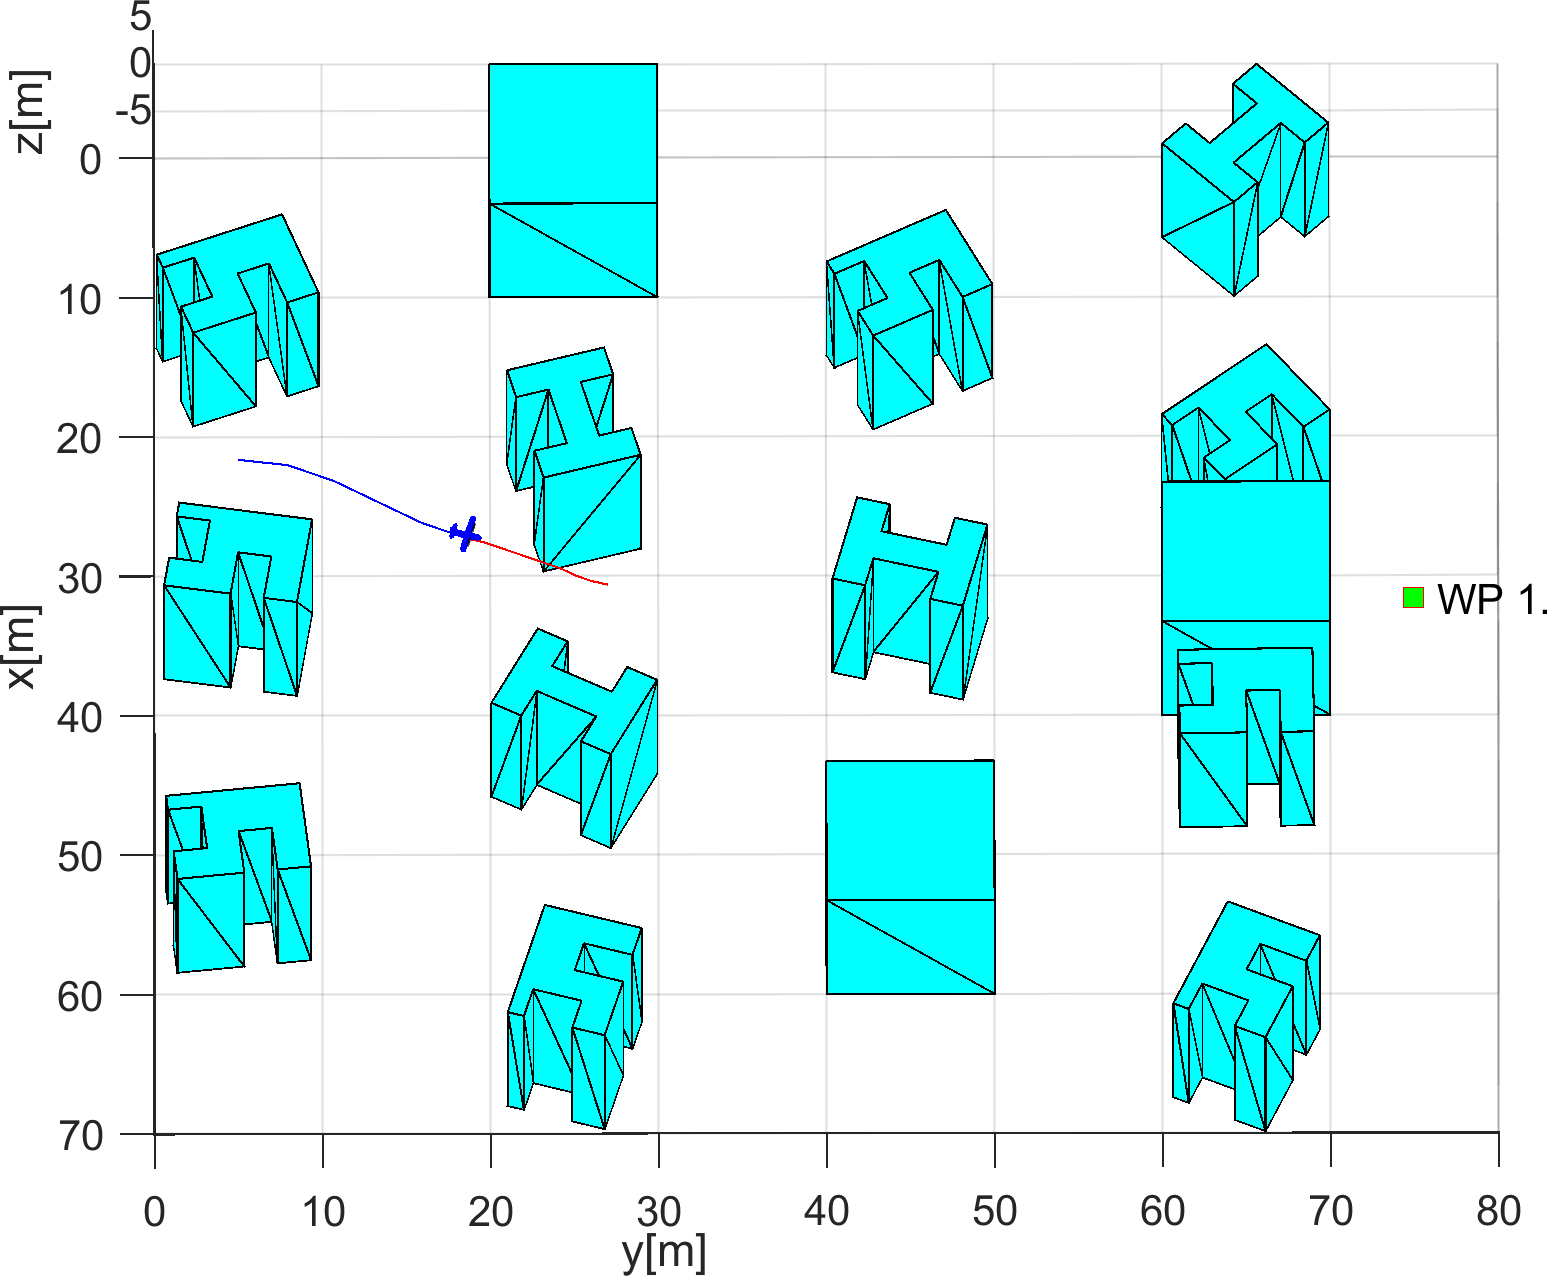
\includegraphics[width=0.9\linewidth]{\FIGDIR/NS007ConstraintsPolynomialSlalom-00015}
        \caption{Open space obstacle.}
        \label{fig:slalomOpenSpaceObstacle}
    \end{subfigure}
    \begin{subfigure}{0.48\textwidth}
    	\centering
        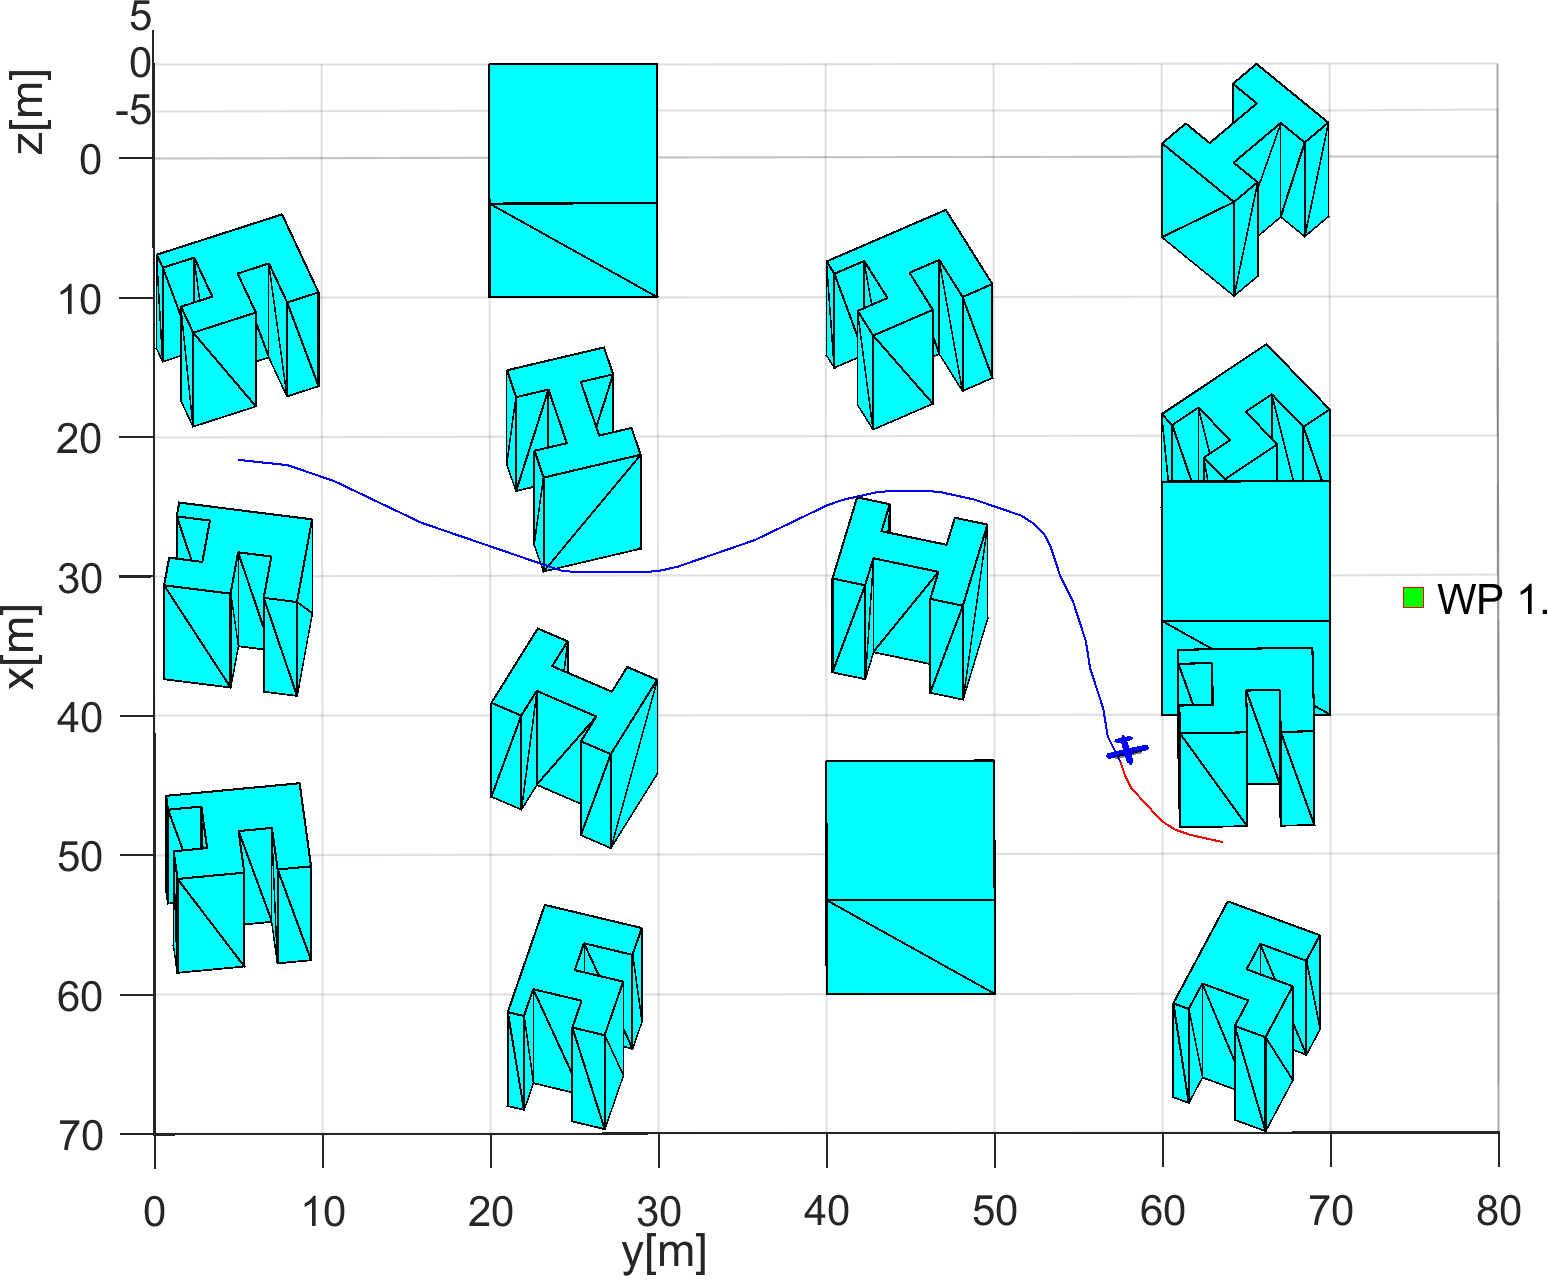
\includegraphics[width=0.9\linewidth]{\FIGDIR/NS008ConstraintsPolynomialSlalom-00069} 
        \caption{Hidden waypoint start.}
        \label{fig:slalomHiddenWaypointStart}
    \end{subfigure}
    \\
    \begin{subfigure}{0.48\textwidth}
	    \centering
        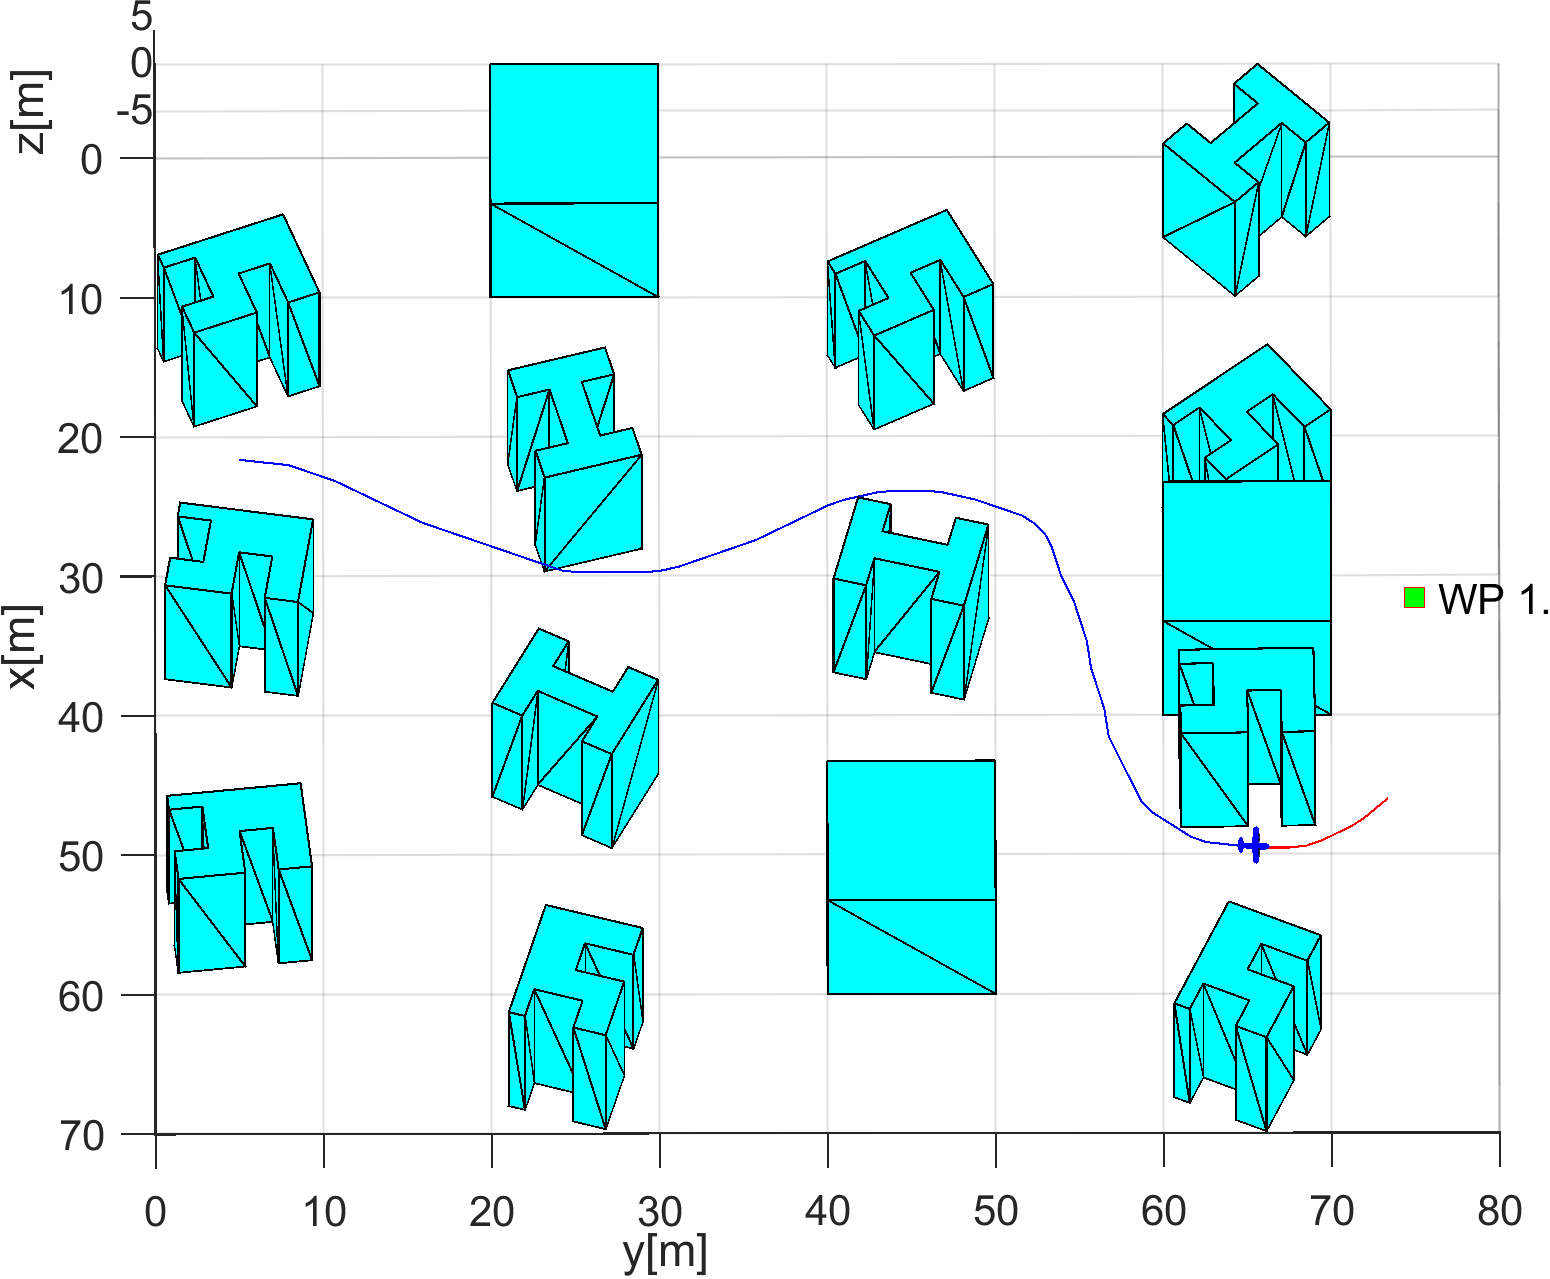
\includegraphics[width=0.9\linewidth]{\FIGDIR/NS009ConstraintsPolynomialSlalom00080} 
        \caption{Hidden waypoint middle.}
        \label{fig:slalomHiddenWaypointMiddle}
    \end{subfigure}
    \begin{subfigure}{0.48\textwidth}
    	\centering
        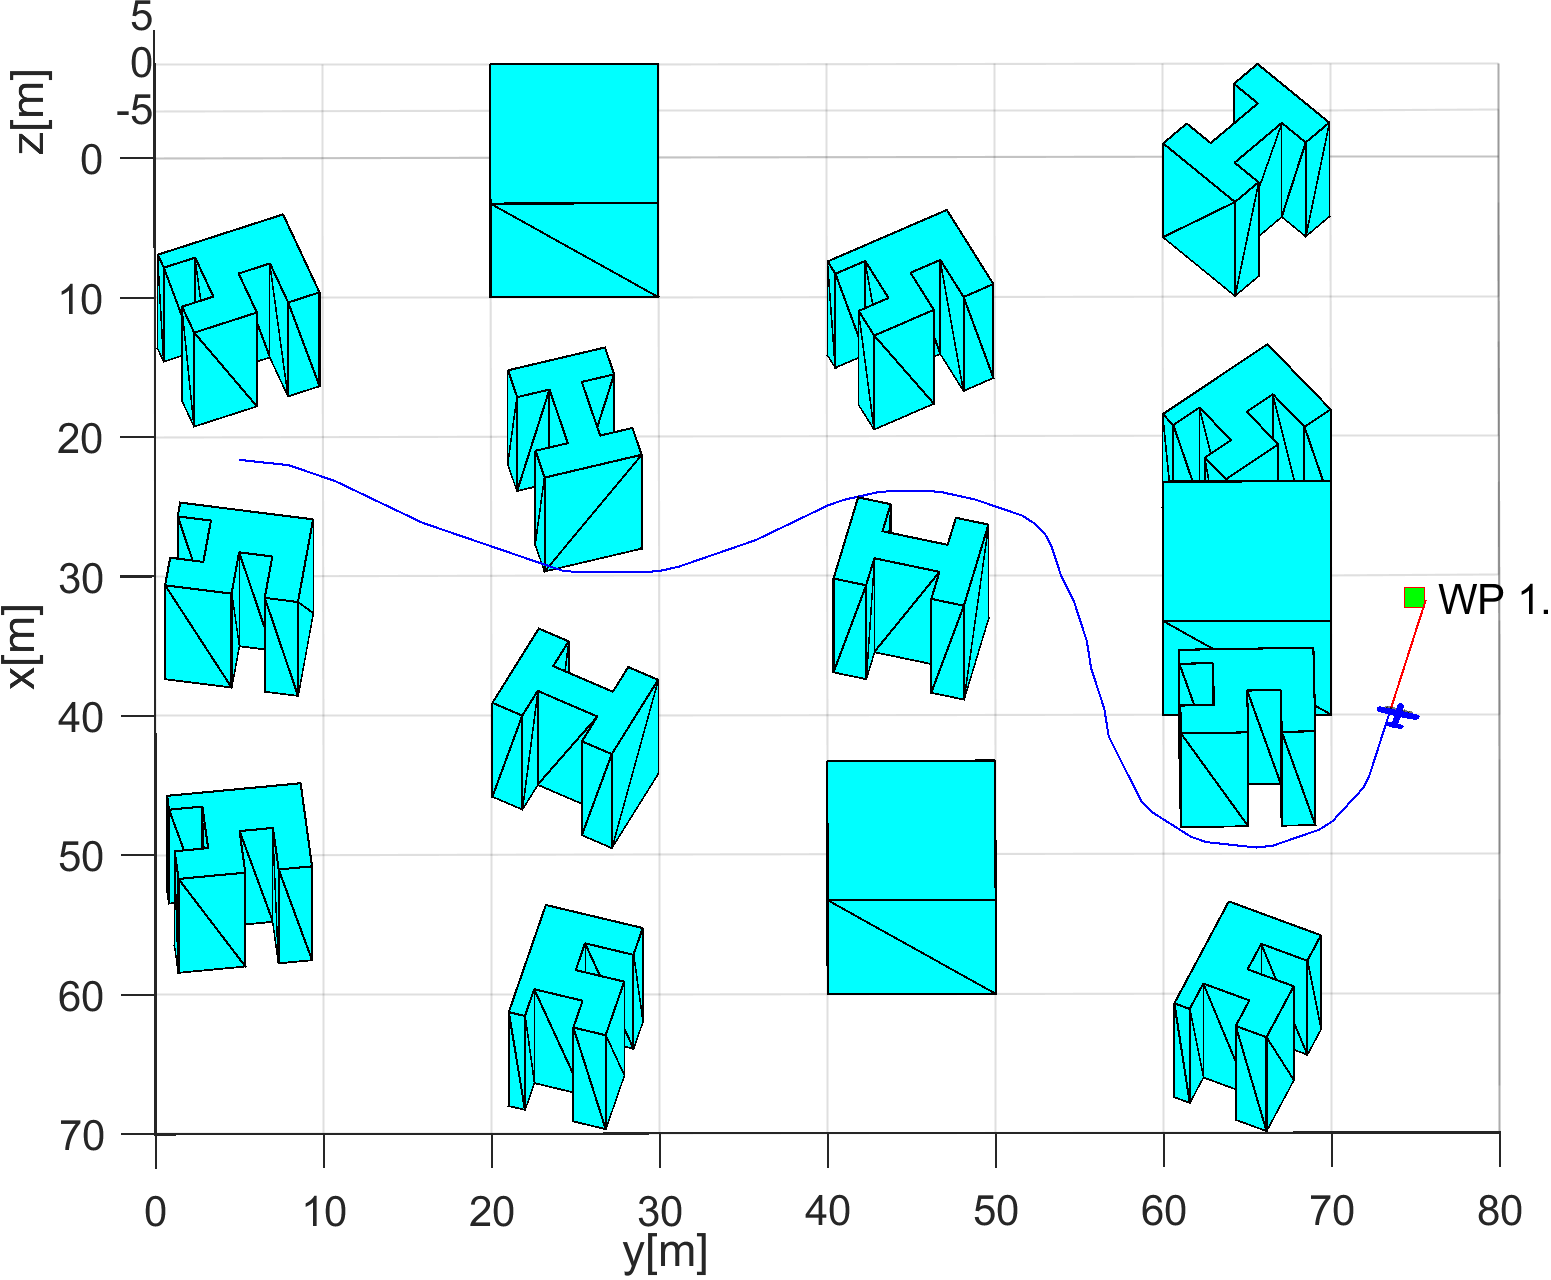
\includegraphics[width=0.9\linewidth]{\FIGDIR/NS010ConstraintsPolynomialSlalom00094} 
        \caption{Hidden waypoint end.}
        \label{fig:slalomHiddenWaypointEnd}
    \end{subfigure}
    \caption{Test scenario for \emph{Slalom} with \emph{hidden waypoint}. }
    \label{fig:testCaseSlalomwithHiddenWaypoint}
\end{figure}


\paragraph{Distance to Body/Safety Margin Evolution:} The \emph{UAS} (blue fill) does not break a \emph{safety margin} (yellow fill) nor \emph{body margin} (red fill) as you can seen in (fig. \ref{fig:testCaseSlalomAvoidancePerformance}). Hindered space is accounted into decision making, because the distance to closest obstacle will never breach \emph{safety margin} (yellow fill). If it was not, the UAS will break \emph{safety} or \emph{body} margin. 

\emph{Body} and \emph{Safety margin} are changing values depending on the \emph{nearest obstacle} and \emph{mutual position of obstacle and UAS}. The ranges of \emph{body} and \emph{safety margins} are reflected in (tab. \ref{tab:obstacleSetSlalom}). 

\begin{figure}[H]
    \centering
    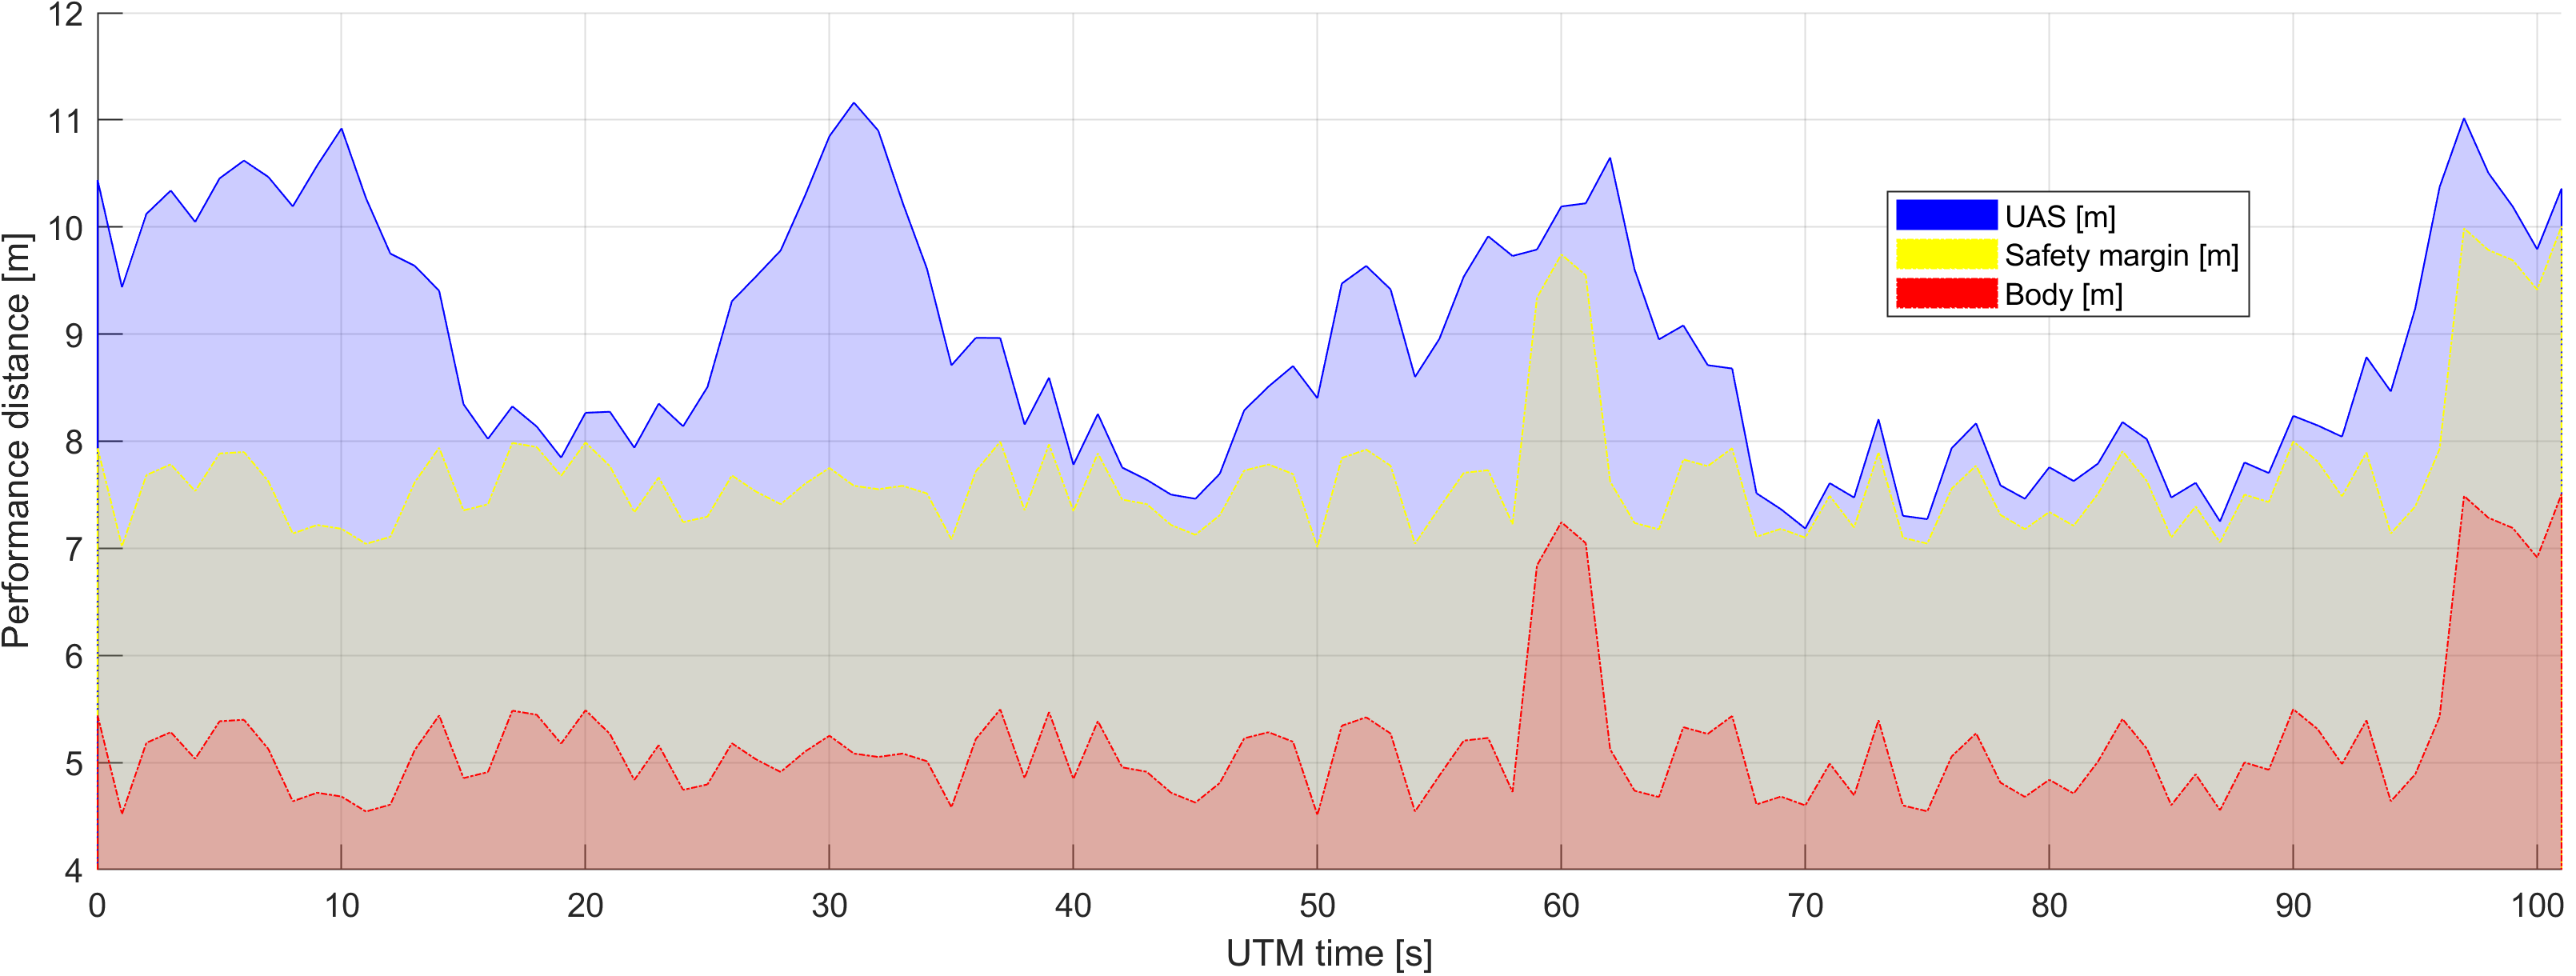
\includegraphics[width=0.8\linewidth]{\FIGDIR/NS011ConstraintsPolynomialSlalomPerformance} 
    \caption{Distance to body/safety margin evolution for \emph{Slalom scenario}.}
    \label{fig:testCaseSlalomAvoidancePerformance}
\end{figure}

\paragraph{Distance to Body/Safety Margin Peaks:} The \emph{UAS} distance to boundary of \emph{safety} and  \emph{body} margin is given in (tab. \ref{tab:testCaseSlalomSafetyAndBodyMarginDistances}). The minimal distance of \emph{UAS border}(blue line) to \emph{safety margin boundary} (yellow line fig. \ref{fig:testCaseSlalomAvoidancePerformance}) is $0.0856$ $m$ which can be considered as marginal $0$. The minimal \emph{body margin} distance is $2.5856$ $m$ which is reflects \emph{safety margin} $2.5$ $m$ at that moment. The condition $safety Margin Distance \ge 0$ holds.
    
    
The difference between minimal and maximal \emph{safety margin distance} is $\sim 3$ $m$ which indicates that mission environment is  tightly packed with obstacles.

\begin{table}[H]
    \centering
    \begin{tabular}{c|c||c}
    \multicolumn{2}{c||}{Parameter} & UAS 1 \\\hline\hline
    \multirow{2}{*}{Distance to Safety Margin} & min & 0.0856\\\cline{2-3}
                                            & max & 3.7391 \\\hline
    \multirow{2}{*}{Distance to Body Margin}   & min & 2.5856  \\\cline{2-3}
                                            & max & 6.2391 
    \end{tabular}
    \caption{Distance to body/safety margin peaks for \emph{Slalom scenario}.}
    \label{tab:testCaseSlalomSafetyAndBodyMarginDistances}
\end{table}


\paragraph{Path tracking performance:} Path tracking is given in (fig. \ref{fig:testCaseSlalomPathTracking}). The line between Starting position (green square, marked S) and  goal waypoint (green square marked 1) is reference trajectory (green dashed line). The flown trajectory (blue solid line) is showing evolution over mission time (Time [s]) in global coordinate frame split into three axes (x[m], y[m], z[m]). The UAS was all time in \emph{Emergency Avoidance Mode} due the vicinity of dangerous obstacles. 

The \emph{UAS} reached final navigation waypoint, which fulfills acceptance criteria. The UAS has taken a significant detour (x[m] evolution) due to hidden \emph{waypoint}. 

The test has been run multiple times to check if \emph{Right-Up} preference for avoidance is always selected. \emph{Small noise} (0.5-1m) was added to obstacle positions. The algorithm always chose similar deterministic path. The higher noise levels were not possible due the obstacle original size (tab. \ref{tab:obstacleSetSlalom}).

\begin{figure}[H]
    \centering
    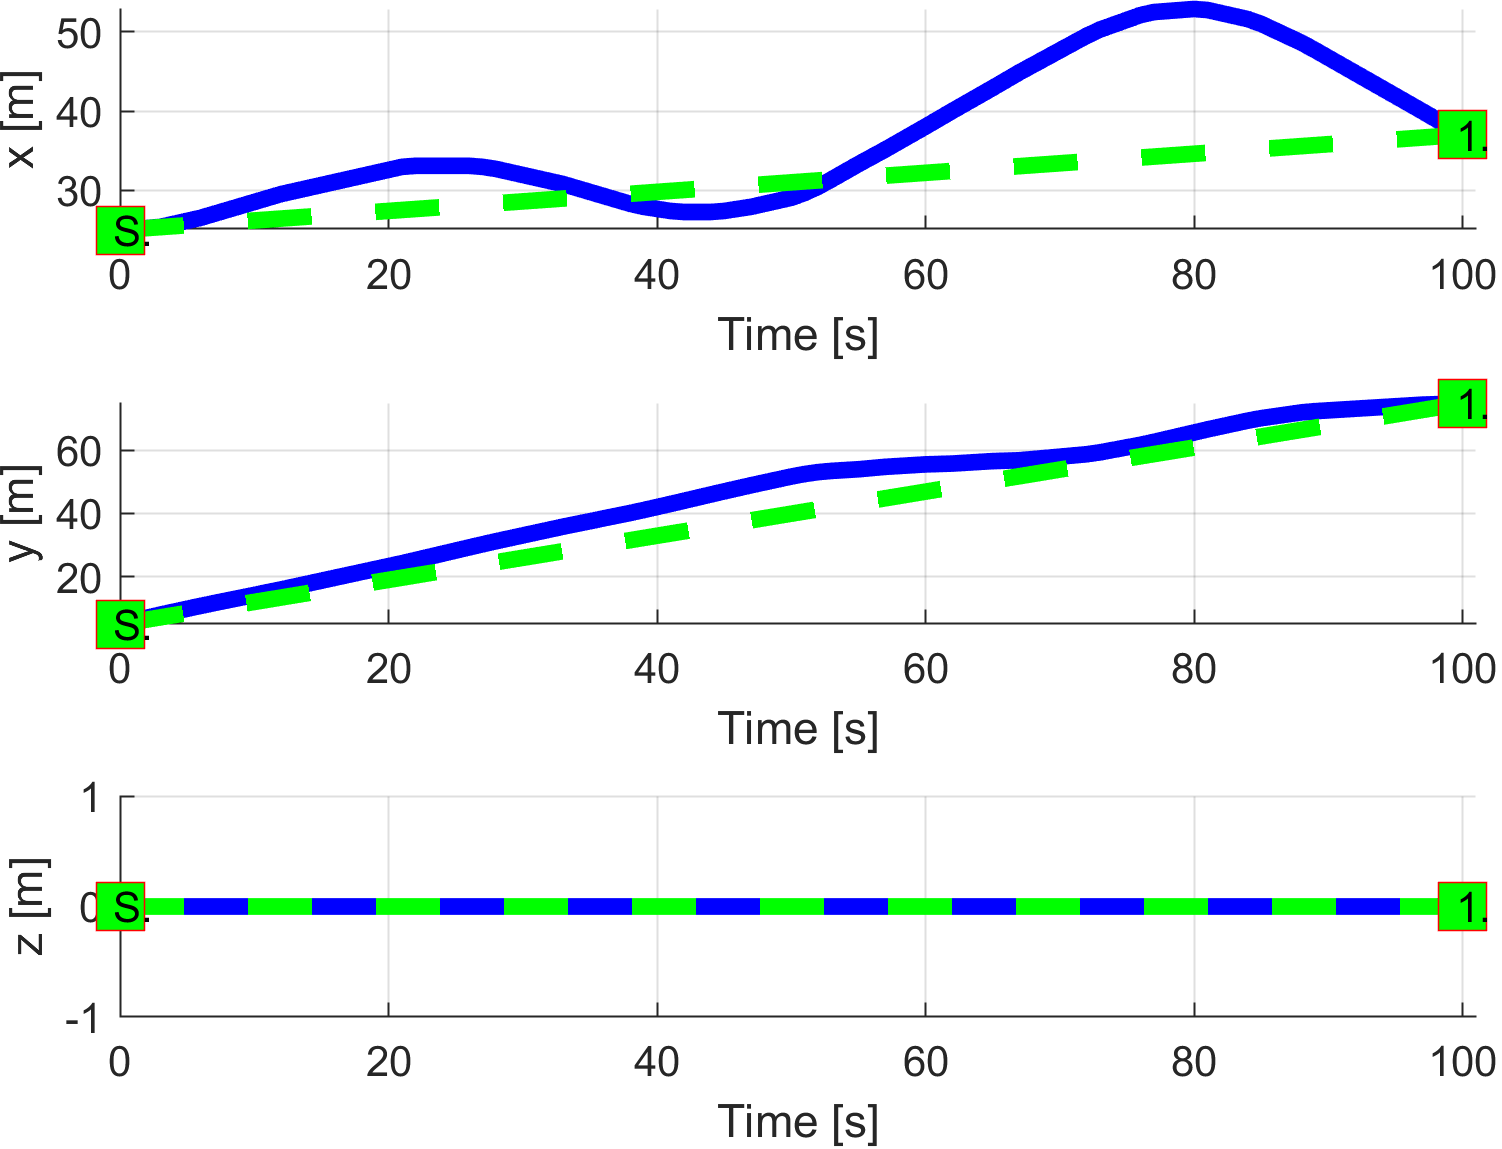
\includegraphics[width=0.55\linewidth]{\FIGDIR/NS012ConstraintsPolynomialSlalomPathFollowing} 
    \caption{\emph{Slalom} path tracking.}
    \label{fig:testCaseSlalomPathTracking}
\end{figure}


\paragraph{Path Tracking Deviations:} Deviations given in (tab. \ref{tab:pathTrackingParametersForSlalomAvoidance}) from \emph{reference trajectory} (fig. \ref{fig:testCaseSlalomPathTracking}) are in expected ranges considering \emph{mission plan} (tab. \ref{tab:missionSetupSlalomScenario}) and \emph{obstacle properties} (\ref{tab:obstacleSetSlalom}).

\begin{table}[H]
    \centering
    \begin{tabular}{c||c}
        \multirow{2}{*}{Param.} & UAS 1\\\cline{2-2}
                        & $\mathscr{WP}_1$  \\\hline\hline
          $\max |x|$    & 17.90      \\\hline
          $\max |y|$    & 12.41    \\\hline
          $\max |z|$    & 0        \\\hline
          $\max dist.$  & 20.06   \\
    \end{tabular}
    \caption{Path tracking properties for \emph{Slalom} scenario.}
    \label{tab:pathTrackingParametersForSlalomAvoidance}
\end{table}

% 02 Slalom scenario
\paragraph{Computation Load:} The \emph{computation load} for \emph{scenario} (fig.\ref{fig:slalomComputationTime}) shows used time (y-axis) over decision frame (x-axis).

The UAS is moving over \emph{semi-clustered} environment the \emph{computation load} is almost constant.

\begin{figure}[H]
    \centering
    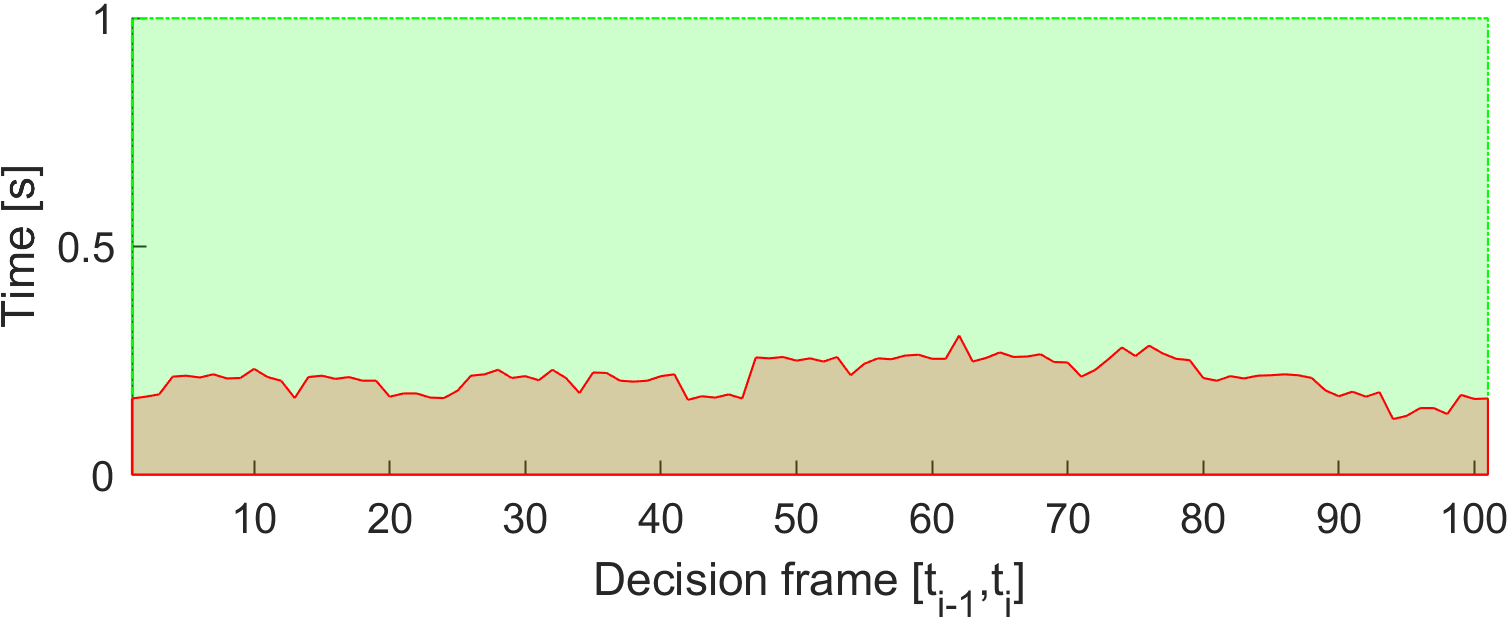
\includegraphics[width=0.65\linewidth]{\FIGDIR/NS093SlalomComputationTime} 
    \caption{Computation time for \emph{Slalom} scenario.}
    \label{fig:slalomComputationTime}
\end{figure}
